In dem folgenden Kapitel sollen die Ergebnisse der Implementierungen ausgewertet und analysiert werden. 

\section{Programmierung}
Zunächst werden einige messbare Zahlen anhand der Implementierung erörtert. 
\TODO{Besserer Name}

\subsubsection{Entwicklungszeitconstraints}
Wenn es um Entwicklungzeit und Fortschritt geht, dann ist oft auch ein Faktor, wie lange die App braucht um gebaut zu werden und wie lange es dauert um Änderungen in der App anzuzeigen. Oft muss man bei der Entwicklung von Oberflächen auch einige Kleinigkeiten ändern und dann überprüfen, ob die Änderung den gewünschten Effekt hatte. Deshalb sind vor allem kurze ladezeiten von Änderungen besonders wichtig.

Für diesen Test wurde die Dauer des erstmaligen Compilieren, die Dauer eines Neubauens auf Basis eines bestehenden Caches, die Dauer bis Layoutänderungen und bis Anwendungslogik geladen wurde, im Debug Modus durchgeführt. Es wurde außerdem die Compilierzeit im Release Modus aufgezeichnet.
Die Tests hierfür wurden jeweils fünf mal ausgeführt und dann am Ende ein Durchschnitt gebildet. Als Hardware wurde ein PC mit 32GB RAM und einer Ryzen 5 2600 6-Kern CPU genutzt. 
Die genauen Zahlen sind immer abhängig von der Hardware und der Appgröße abhängig, geben aber einen Einblick ob hier einzelne Ansätze einen Vorteil haben. 

\begin{table}
\centering
\caption{Dauer typischer Entwicklungsoperationen in Sekunden}
\begin{tabular}{ |p{4cm}||p{3cm}|p{2cm}|p{2cm}|p{3cm}|p{3cm}| }
 \hline
 Funktion & Flutter-Hybrid & Flutter & Kotlin-Nativ & Kotlin-WebView \\
 \hline
 Build Zeit Release       &   59,2&   54,22& 40,92& 22,42\\
  \hline
 Build Zeit Debug  & 33,78& 28,76& 20,2& 20,19\\
  \hline
 Erneuter Build mit Cache & 8,8& 8,36& 3,36& 3,21\\
  \hline
 Neuladen nach Layoutänderg & 0,59& 0,6& 2,59& 2,64\\
  \hline
 Neuladen nach Logikänderung & 0,626& 0,622& 3,18& 2,63\\
  \hline
\end{tabular}
\label{tab:evaluations_build_time}
\end{table}

Bei der Analyse der Daten fällt auf, dass grundsätzlich bei der Build Zeit die Flutter Apps schlechter abschließen. Sowohl beim erstellen einer Release oder auch Debug APK sind die Kotlin Applikationen schneller. Bei der Debug APK ist die Sache jedoch nicht so ein großer Unterschied und selbst die Kotlin-WebView App benötigt gleich lang wie die reine Kotlin Implementierung. Beim compilieren einer Release App scheint es tatsächlich mehr um den Umfang der Applikation zu gehen, als bei der Debug Version.
Der auffälligste Unterschied ist jedoch die Neuladezeit nach einer Änderung im Quellcode. Denn Flutter mit dem HotReload Feature schneidet hier deutlich besser ab und benötigt somit gerade mal 1/5 der Zeit die die mit Koltin implementierten Applikationen benötigen. Dazu kommt, dass beim Neustarten bei Android, man an den Anfang der Applikation zurückgesetzt wird, während bei Flutter man an der aktuellen Stelle bleibt und somit nicht erst wieder durch die Anwendung gehen muss. Dadurch ändert man etwa ganz einfach die Farbe eines Textes im Fluttercode und bekommt innerhalb von 600ms die Änderung angezeigt. So sparrt man nicht nur Zeit, sondern kann sich auch besser darauf konzentrieren, eine ordentliche Nutzeroberfläche zu entwickeln.

\subsubsection{Performance}


\begin{table}
\centering
\caption{Performancemessung der verschiedenen Applikationen }
\begin{tabular}{ |p{4cm}||p{3cm}|p{2cm}|p{2cm}|p{2cm}|p{2cm}| }
 \hline
 Parameter & Flutter-Hybrid & Flutter & Kotlin-Nativ & Kotlin-WebView \\
 \hline
 Durchschnittliche CPU-Auslastung       &   2,54\%&   1,96\%& 0,9\%& 1,8\%\\
  \hline
 Maximale CPU- Auslastung  & 9,8\%& 6,4\%& 3,6\%& 7,4\%\\
  \hline
 Durchschnittliche RAM-Auslastung & 215,38 MB& 150,68MB& 86,74MB& 107,68MB\\
  \hline
 Maximale RAM- Auslastung & 238MB& 175,46MB& 100,64MB& 117,06MB\\
  \hline
 App-Größe & 8,6MB& 8,4MB& 5,2MB& 4,4MB\\
  \hline
 Maximale Startzeit & 532ms& 452ms& 263ms& 486,6ms\\
 \hline
 Durchschnittliche Renderzeit &8,68ms& 5,12ms& 9,04& 21,88ms\\
 \hline
\end{tabular}
\label{tab:evaluations_performance}
\end{table}

In Tabelle \ref{tab:evaluations_performance} sieht man die Ergebnisse von Performance Messungen, die an den beschriebenen Implementierungen durchgeführt wurden.
Die Messungen wurden mit dem Programm Apptim durchgeführt. Dies zeichnet die Performance von Apps während der Nutzung einer App auf. Die Tests wurden auf einem Google Pixel 5 durchgeführt mit Android Level 12 oder auch API Level 31. Es hat dabei 8GB DDR4-Ram und einer 8-Kern-CPU, die mit 6x1,8GHz, 1x2,2GHz und 1x2,4GHz getaktet sind.
Der Test wurde dabei für jede Implementierung 5 mal wiederholt und aus den Ergebnissen dann ein Durchschnittswert gebildet. Die Apps wurden nach jeder Nutzung zurückgesetzt und alle anderen Apps wurden während der Tests beendet. Die Apps waren dafür jeweils als Release-Version installiert, so dass die Apps bei bester Leistung wie auch bei einem Endbenutzer laufen würden.
Renderzeit entspricht der Zeit, die gebraucht werden, bis die Änderungen geziechnet wurden und als Bild angezeigt werden können

Was man hierbei beobachten kann ist, dass die native Android App insgesamt die schnellste ist, während die Hybride Flutter App die am schlechtesten performende. Die schnellste Renderzeit hatten die Flutter-Applikationen, während die Auslastung des Rams bei den Android Applikationen deutlich geringer war. Überraschend zu sehen ist, dass die WebView Applikation mehr Ressourcen verbraucht als die nativ implementierte, obwohl sie lediglich einen WebContainer bauen muss. was außerdem auffällt, ist dass Flutter Applikationen etwa zwei mal so groß sind als die nativen. Eine weitere Sache ist, dass die die Android Apps und die reine Flutter App sehr vergleichbar sind, während die Hybride Flutter App in fast jeder Kategorie doppelt so viele Ressourcen verbraucht hat, wie die native Android Anwendungen.

Was festhalten werden kann, ist, dass eine Flutter App zwar in der Performanz etwas den nativen geschriebenen Applikationen hinterherhängt, jedoch der Unterschied nicht derart groß ist, als dass er eine große Rolle spielen würde. Was jedoch auffält ist das die hybride Flutter App Performance technisch deutlich schlechter abschneidet als die native.  

Biorn Hansen et al\cite{BirnHansen.2020} sagen in ihrer Auswertung, dass sie einen deutlichen Anstieg bei Datenbankbenutzung sehen konnten. Deshalb wurde bei der Flutter App und der nativen Android App  jeweils eine Datenbankimplementierung nach der Dokumentation der einzelnen Plattformen eingefügt. Daraufhin wurden beide Apps wieder wie oben beschrieben getestet und am Ende der Anstieg in den einzelnen eine Applikationen ausgewertet und in Tabelle \ref{tab:evaluations_performance_Overhead_database} zusammengetragen.

Auffällig ist, dass die CPU auslastung bei beiden gleichmäßig ansteigt, während bei der Nativen die RAM Nutzung deutlich mehr ansteigt, als bei der Flutter. Wenn Tabelle \ref{tab:evaluations_performance} miteinbezogen wird, nutzt die native App damit immer noch weniger Ram als die normale Flutter, da diese bereits ohne Datenbank eine recht hohe RAM Nutzung hat. Bei der App Startzeit ist die Flutter App, die nochmal 60 ms mehr länger braucht als die Android und somit nun 36\% langsamer ist als die Native. Bei der Renderzeit zeigt sich weiterhin die stärke von Flutter, da hier ein deutlich geringerer Anstieg zu verzeichnen ist.

\begin{table}
\centering
\caption{Unterschied bei Implementierung mit zusätzlicher Datenbankimplementierung}
\begin{tabular}{ |p{7cm}||wc{3.5cm}|wc{3.5cm}|}
 \hline
 Parameter & Flutter &  Kotlin-Nativ \\
 \hline
 Durchschnittliche CPU-Auslastung       &  0,44\%&   0,26\%\\
  \hline
 Maximale CPU-Auslastung  & 2,2\%& 2,6\%\\
  \hline
 Durchschnittliche RAM-Auslastung & 5,64 MB& 18,04MB\\
  \hline
 Maximale RAM-Auslastung & 4,98MB& 39,64MB\\
  \hline
 App-Größe & 0,1MB& 0,1MB\\
  \hline
 Maximale Startzeit & 221ms& 162,6ms\\
 \hline
 Durchschnittliche Renderzeit &0,82ms& 4,68ms\\
 \hline
\end{tabular}
\label{tab:evaluations_performance_Overhead_database}
\end{table}

Grundsätzlich kann man eigentlich festhalten dass native Entwicklungen meistens die beste Performance haben werden, Jedoch ist mit Flutter ein Framework auf den Markt gekommen, das diese Einstellung stark ins wanken geraten. Denn Flutter ist wie bereits erwähnt ein Framework, dass den geschriebenen Dart-Code in Nativen Code umwandelt. Es hat sich außerdem zum Ziel gesetz, möglichst performant zu sein. Eine Untersuchung von Biørn-Hansen et Al hat ergeben, das Nativ zwar immer noch am performantesten ist, und Flutter da in einigen Kategorien doch noch hinten dran ist. Sie stellten jedoch fest, dass gerade bei ausführen von Aufgaben Flutter weniger Speicher benötigt und ansonsten grundsätzlich durchschnittlich abschloss \cite{BirnHansen.2020}. 
Eine andere Untersuchung zeigte, dass  es darauf ankommt, was man macht

\subsubsection{Debugging/Testing}

\section{Community \& Dokumentation}
Die Entwickler Community ist ein wichtiger Faktor für die Wahl eines Frameworks. Wenn es keine Community gibt, wird es schwer Entwickler oder auch Lösungen für Probleme zu finden, ohne sie selber zu entwickeln. Aber nicht nur Bibliotheken helfen dabei, schneller zu entwickeln sondern auch Frage-Antwort Communities wie Stackoverflow\footnote{https://stackoverflow.com/}.  Die genauen Zahlen der Community-Größe oder die Populärität sind dabei nicht genau bestimmbar. Sie können jedoch anhand einiger Faktoren annähernd bestimmt werden, bzw. verglichen werden.

\subsubsection{Star-History}
Ein erster Anhaltspunkt ist die Sogenannte Star-History von Github-Repositorys. Es gibt an, wie viele Leute sich die Repositories mit einem Stern markiert haben. Es gibt weniger absolute Zahlen an, wie viele Leute mit einem Framework oder Programmiersprache entwickeln, es zeigt jedoch ganz gut wie viel Interesse Leute an der Entwicklung dieser haben.
\begin{figure}[ht]
  \centering
  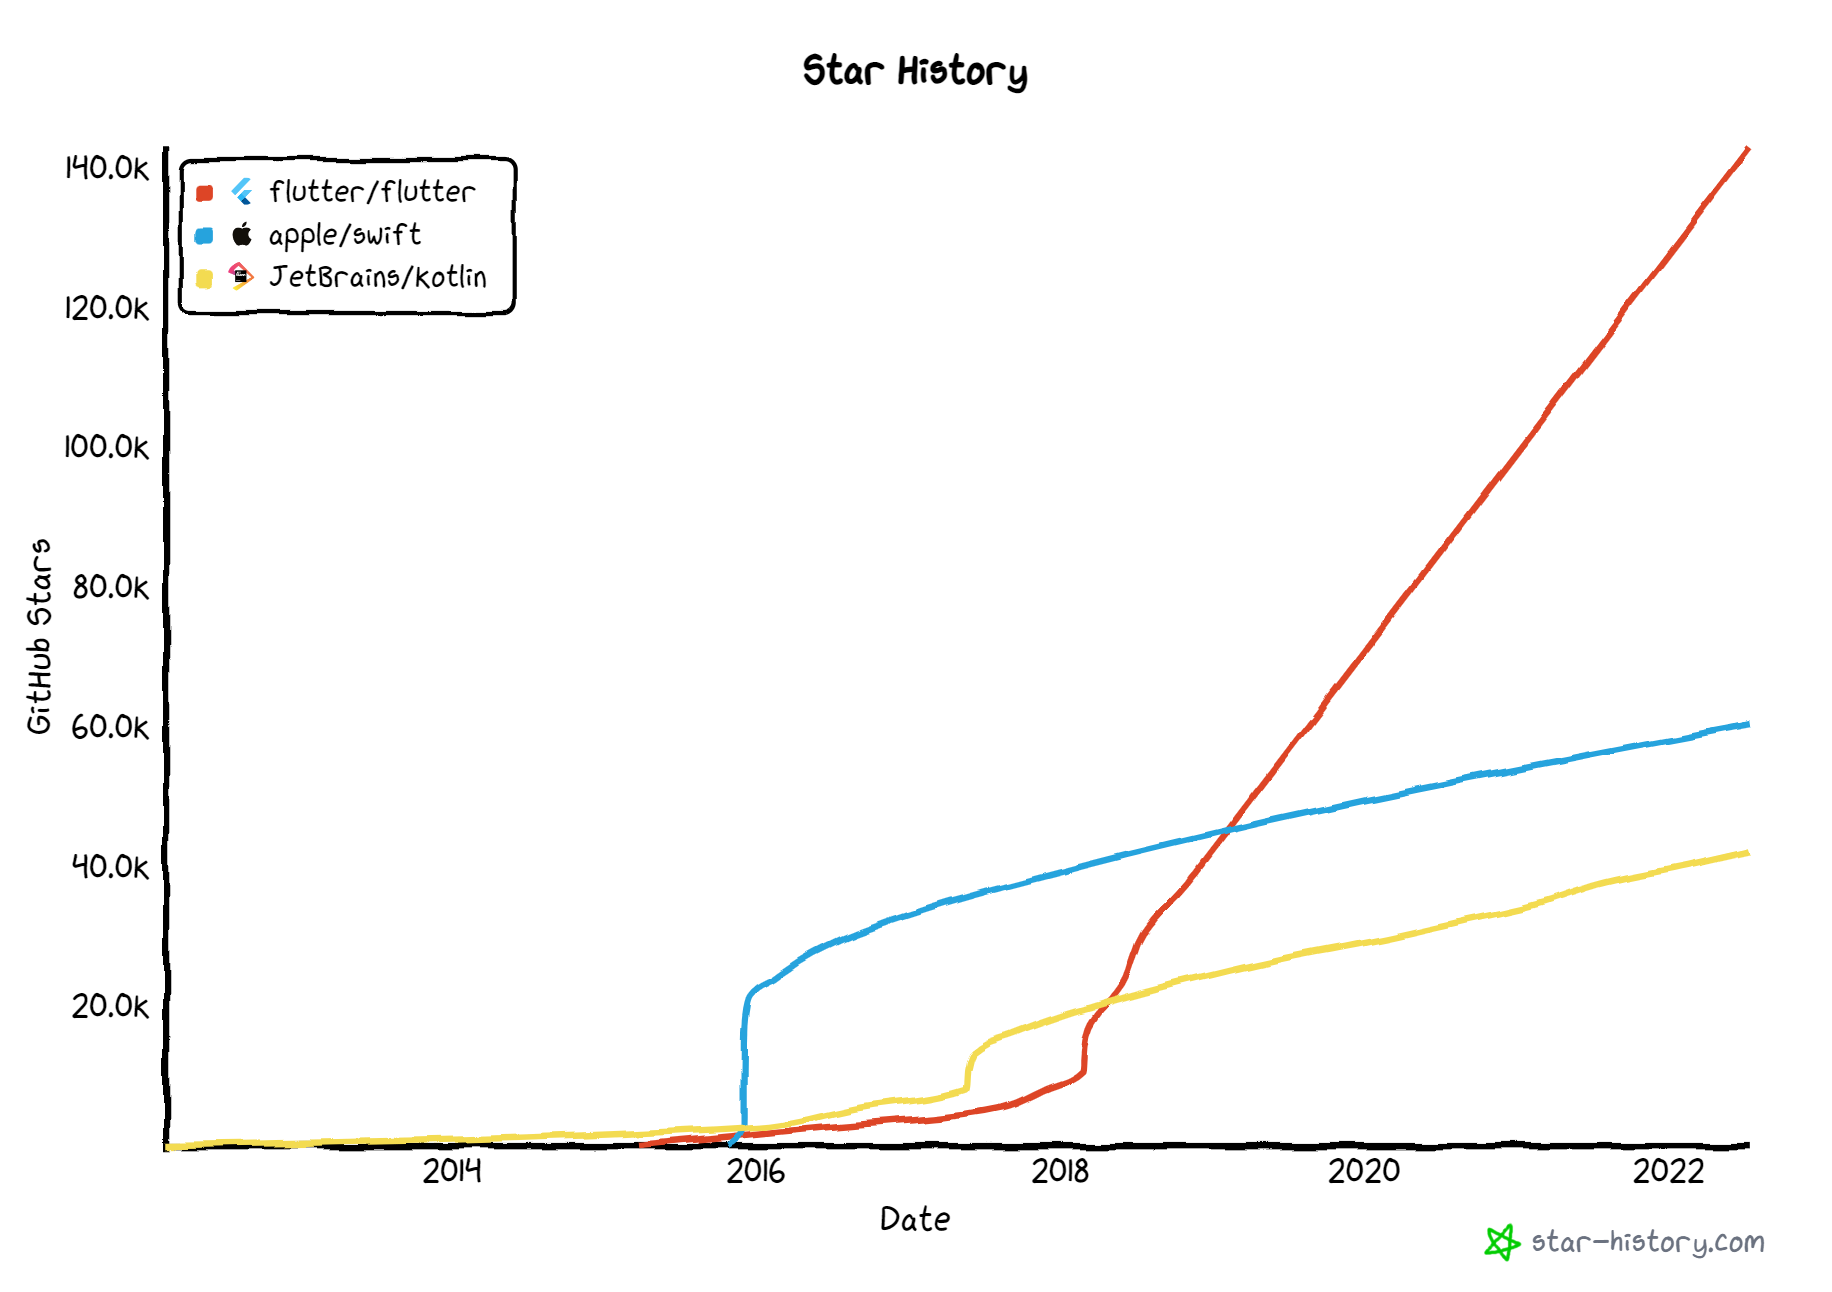
\includegraphics[height=7cm,keepaspectratio]{images/star-history_programming languages.png} 
  \caption[Zeitlicher Verlauf von Stars der Github-Repositorys von Swift, Kotlin und Flutter]{Zeitlicher Verlauf von Stars der Github-Repositorys von Swift, Kotlin und Flutter\protect\footnotemark }
  \label{fig:start_history}
\end{figure}
\footnotetext{https://star-history.com/\#flutter/flutter\&JetBrains/kotlin\&apple/swift\&Date}




\section{Sonstiges}
\subsubsection{Maintainability, Scalibility, Testability}
\subsubsection{Plattformabdeckung}
\subsubsection{Programmieraufwand}
\subsubsection{Verfügbarkeit  von Änderungen}
\subsubsection{Offline Funktionalität}




Mögliche Kriterien:
The comparison investigates several aspects of each language, including program length, programming effort, runtime efficiency, memory consumption, and reliability
siehe:https://ieeexplore.ieee.org/abstract/document/876288

Ease of Coding, Debug/Test, Distribution/Upgrade, Ease of Use: Download, Install and Update, User Interface, Functionalities, Performance Comparison 
siehe:https://ieeexplore.ieee.org/abstract/document/8082717

-----
Vortrag zu Cross Plattform Notizen:

Flutter ist für Ubuntu Standardsprache zur Desktopanwendungsentwicklung

Mittlerweile für fast alle möglichen Plattformen übersetzbar und Gemeinschaft sehr aktiv.

Es gibt eigentlich keine richtigen Gründe mehr nativ zu entwickeln. Mit Flutter ist quasi alles umsetzbar, was man will und wenn es noch nicht das benötigte Plugin gibt, so kann man es selbst entwickeln. Das kann zwar etwas kompliziert werden, aber von der Sache her nicht ummöglich.

Bei Flutter kann man Plugins schreiben. Diese funktionieren, indem man einen Dart Code schreibt und die entsprechenden nativen Codeteile. Dadurch weiß der Dart-Compiler wie er den DartCode in die verschiedenen nativen Anwendungen übersetzt.

Die Grundfunktionalität von Flutter funktioniert, indem ein Canvas genommen wird, auf den die verschiedenen UI-Komponenten "drauf" gemalt werden. Mit einer dahinter liegenden Zuordnung und Tracking wird es dann zu einer funktionalen Nutzeroberfläche.

------------Frage: Ist es überhaupt noch sinnvoll, eine App nativ zu entwickeln? Macht es nicht immer mehr Sinn eine Cross-Plattform-Entwicklung zu tun, falls man einmal doch auf eine weitere Plattform umsteigen will? 
Es könnte ja immer sein, dass man die App erweitern kann. Dann müsste man eine zusätzliche Entwicklung bezahlen. Man müsste gewissermaßen komplett von vorne anfangen. Während wenn man bereits in Flutter etwa entwickelt hat, muss man nur noch die benötigte Plattform kompilieren und eventuell ein paar Sachen anpassen. 

Andererseits hat man einen schnell sich ändernden Technologiemarkt. Flutter wurde erst 2017 auf den Markt gebracht und ist 2021 zum Führenden Framework aufgestiegen. Andererseits ist React Native von einem der viel versprechendsten Frameworks seit dem Erscheinen von Flutter auf dem Abeseigenden Mast und andere haben ganz und gar Ihre Bedeutung verloren.Etwa Apache Flex. Das auch seit 2017 nicht mehr weiter entwickelt wird. So zeigt sich, dass die Wahl auf das richtige Framework und die richtige Entwicklungsstrategie eine sehr wichtige ist und mit viel Vorsicht getroffen werden muss.

-----

Vielleicht ist es gar nicht so sonnvoll feste Kriterien zu finden an denen man die Entwicklung an sich bewerten kann, sondern eher das Endergebnis. Es ist ja auch keine Bewertung sondern eher ein Vergleich.
Kriterien sind:
-Programmlänge
-Programmieraufwand
- verfügbarkeit
-Verfügbarkeit von Hilfestellungen und Fragen und Antworten
- Code lesbarkeit[1]
- Einfachheit[1]
- Datentypen[1]
- Syntax[1]
- Designed to make it impossible to making (some) stupid mistakes? [1]
- Programmierfähigkeiten während Entwicklung ohne ständiges neu Compilen und schnelles Testen     von Sachen[1]
- Possibilitys for reusability and dry code[1]
- A language may be wonderful and amazing and increase developer productivity, but if no talented people are out there that know the language, how will you hire the best team?[1]
- Keine Änderung von Grundsätzlichen Strukturen und Funktionalitäten.

- In general, we think you can write good software in Java, C\#, Python, PHP, or any other myriad languages. You can also write really bad software using any of those. To us, the adherence to widely accepted design principles and philosophies is more important than the specific language.[3]



Quellen hierzu:
-Medium Leseliste
-[1] https://cs.lmu.edu/~ray/notes/evaluatingprogramminglanguages/  , Loyola Marymount University website
-[2]https://easyexamnotes.com/p/language-evaluation-criteria-ppl.html
-[3] https://www.27global.com/how-to-choose-a-programming-language/
- [4]https://journals.plos.org/plosone/article?id=10.1371/journal.pone.0088941
- [5]\url{https://books.google.de/books?id=XUqqCAAAQBAJ&lpg=PR6&dq=criteria%20for%20evaluating%20programming%20languages&lr&hl=de&pg=PA35#v=onepage&q&f=false}

------
Framework Kriterien:

Quellen:
- [1] https://symfony.com/ten-criteria
- [2]


- Popularität und Community Größe: Je mehr genutzt und bekannt, umso mehr evolution und besserwertige und mehr Plugins und Lösungen [1]

- Philosophy: Ein von Profis für diesen Zweck entwickeltes Framework passt besser zu eigenem Projekt während Entwicklung für Framework für sehr spezielle Sachen eher unnützlich [1]

- Langlebigkeit: Wenn ein Framework kurz vor Ende ist oder schon lange keine Updates mehr erhalten hat, so wird es eventuell keine Große Hilfe im meistern zukünmftiger Probleme sein [1]

- Technische Details: Frameworks, die sich an die technischen Standards halten, helfen, nicht zu sehr an speziellen Lösungen eines Frameworks hängen zu bleiben und auch offen für neue Programmiersprachen und Frameworks zu bleiben [1]

- Sicherheit: Frameworks müssen bestimmte Sicherheitsrichtlienien erfüllen. [1]

- Gute Dokumentation: Eine gute Dokumentation durch den Entwickler ist entscheidend um verlässliche Informationen zu erhalten [1]

-Lizenzen: Bei Programmiersprachen wie Java gibt es einige Versionen die nur mit gekaufter Lizenz nutzbar sind. Darüber sollte man sich klar machen, bevor man eine Entscheidung trifft. Es ist grundsätzlich kein schlechtes Zeichen, muss allerdings beachtet werden. [1]

- Entwicklerverfügbarkeit [1]

-Ausprobieren:Wenn man nicht mit dem Framework zurecht kommt, sollte man eventuell ein anderes versuchen. Nur durch ausprobieren erfährt man wie gut man damit entwickeln kann.[1]
